\chapter{骨髓血细胞检测与识别软件设计}
本节介绍基于深度学习的骨髓血细胞检测与识别软件的设计。首先分析了软件的需求,包括了功能性需求
与非功能性需求。接着,介绍了软件的架构设计与各个模块的流程图与数据库表设计。软件模块包括了用户登录注册模块、骨髓血细胞检测模块、
骨髓血细胞识别模块、患者数据管理模块与日志模块。最后展示了软件实际实现的功能界面,并设计相关测试用例对软件功能进行测试。


\section{需求分析}
本节的目的是实现一个骨髓血细胞自动化检测识别软件,通过第三、四章介绍的深度学习算法将血细胞硬件采集设备收集的图像自动完成血细胞的定位、分类计数。
最终根据FAB分类标准给出病情的诊断。本软件主要解决人工镜检流程复杂、枯燥、主观性强等问题。医生可以将患者数据一键上传,在患者信息管理界面可以查询
相关患者的单张血细胞图像分类结果与整体血细胞分布的柱状图,此外还可以对错分类的血细胞重新进行标注。上述血细胞数据均落入到云端的数据库中,通过数据的不断积累,
未来可以进一步提升模型的识别性能。

\subsection{功能需求分析}
骨髓血细胞检测识别软件包含以下的几种功能,用户登录/注册功能、骨髓血细胞图像上传/检测功能、骨髓血细胞图像识别功能、
患者数据管理查看分析功能。

\textbf{1)用户登录/注册功能}

软件的首页为登录页,用户只有登录后才能使用网站的全部功能。注册用户仅为医院医生,注册后可以使用骨髓血细胞检测、
骨髓血细胞识别功能,并能对检测识别结果进行修订与更改。医生注册后可以对个人信息如昵称、电话、邮箱、部门、性别进行修改。

\textbf{2)血细胞检测功能}

医生输入患者的ID后,将扫描设备拍摄的骨髓血细胞数字化图像上传,上传后图像可在界面实时显示,并展示检测到的血细胞切片,
提供切片图像压缩包下载的功能。在检测精度方面,交并比(IOU)为0.75时,检测的平均精度(AP75)不低于0.90。
在IOU阈值为0.50~0.95时,检测平均精度(AP50:75)不低于0.85。


\textbf{3)血细胞识别功能}

医生在输入患者ID后,选择切片图像上传,软件可以将识别的结果呈现给医生。在识别精度方面,整体分类正确率不低于0.90
针对常见的骨髓血细胞类型如嗜中性粒细胞,淋巴、红细胞的f1-score大于0.95。

\textbf{4)患者数据管理分析功能}

医生可以搜索某患者的骨髓血细胞图像切片,并展示算法识别的类别,医生可以对血细胞识别的类别进行修改,并人工确认。
软件可以对患者的血细胞类别数量分布以直方图或饼状图的形式进行展现,根据FAB标准对血液疾病类型给出初步诊断结果。

\subsection{非功能需求分析}
软件的非功能性需求主要包含以下几个方面。1)性能与速度,需要每小时可完成20张涂片约2000个骨髓血细胞的检测与识别。
2)数据安全性与可靠性,数据计算时,需要保证算法的正确与稳定性,使用数据库维护与更新数据,保证数据的完整性和可追溯性。
3)软件的稳定性,软件在使用中不会因为某些异常或错误而崩溃或无法正常运行。4)软件的易用性,软件的界面与交互设计应该用户友好,
用户能够方便的使用软件骨髓血细胞检测识别任务。5)软件的可扩展性,有清晰的模块化与接口化设计,可以方便的进行检测识别算法的升级。
架构上采用可扩展的架构,可方便的支持新增功能。

\section{软件设计}

\subsection{软件架构设计}
骨髓血细胞检测与识别软件开发使用的技术框架为B/S架构。开发环境为Windows 10、前端使用Vue框架与Element UI组件库。
后端使用的框架Django 2.4、深度学习模型部署工具ONNX、数据库为Mysql 8.0。

\begin{figure}[htbp]                     
  \centering                      
  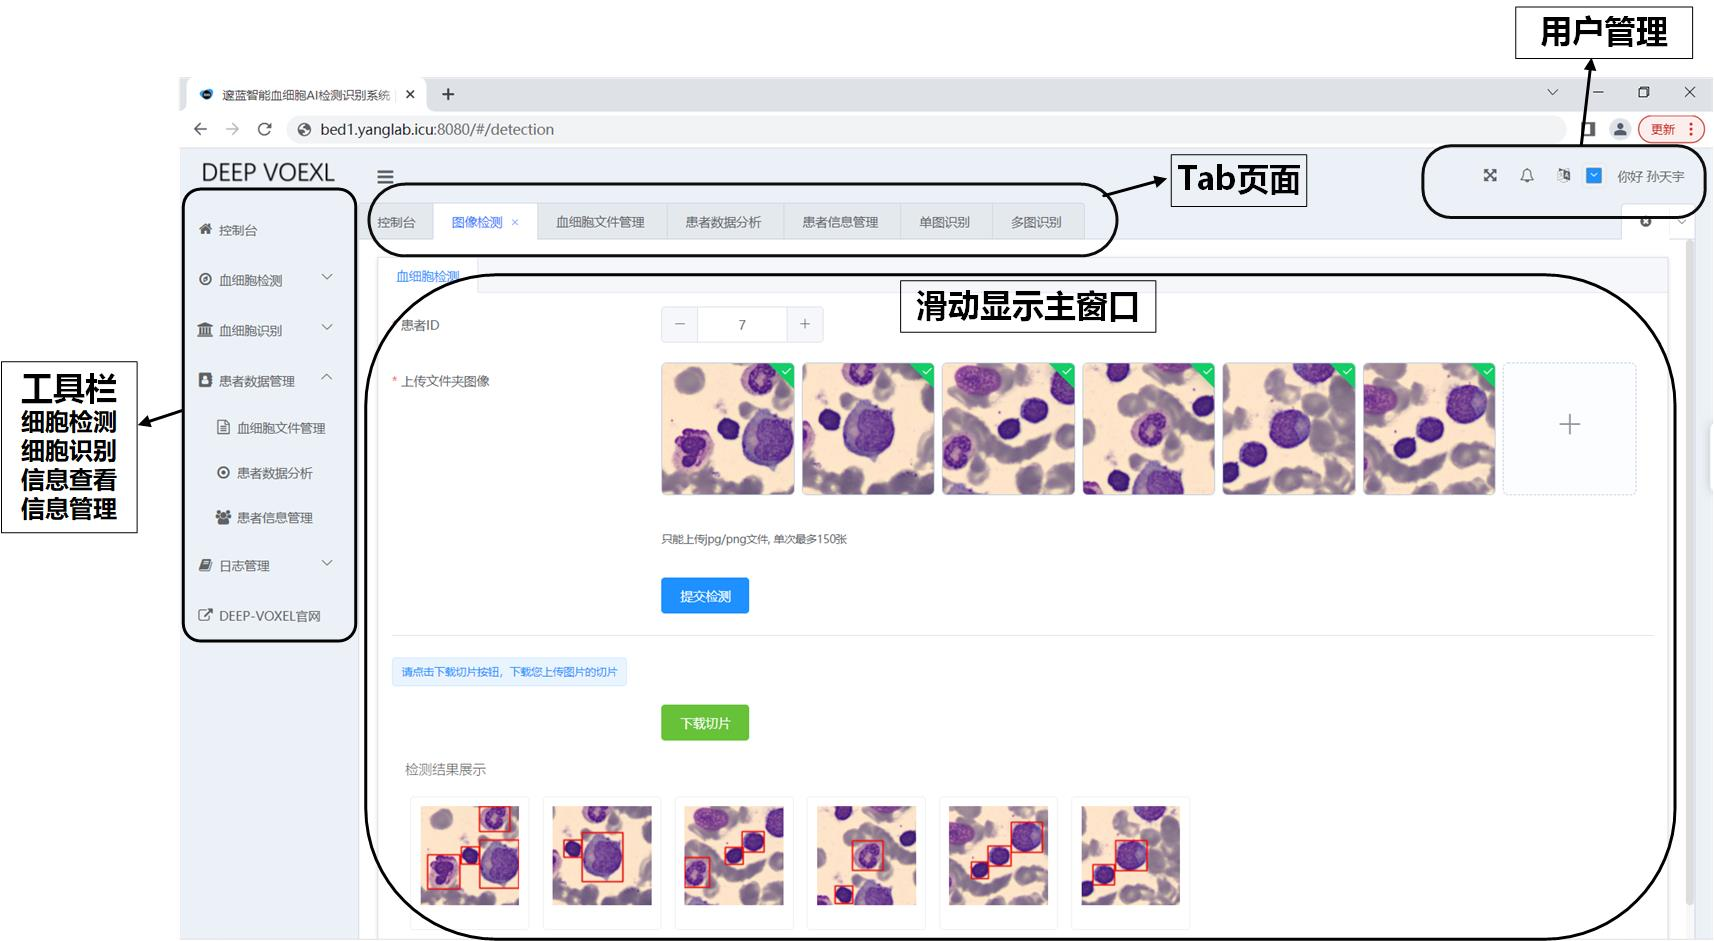
\includegraphics[width=0.99\linewidth]{software.jpg}                      
  \caption{骨髓血细胞检测识别软件架构图}                      
  \label{fig:software}       
\end{figure}

骨髓血细胞检测识别架构如图~\ref{fig:software}所示,根据用户需求分析,主要划分为四个模块分别是用户模块、骨髓血细胞检测模块、
骨髓血细胞识别模块与患者数据管理模块。

软件采用前后端分离的架构,分别进行独立开发与部署。前端与后端的数据交互与通信使用axios网络请求库。
后端服务部署在GPU服务器上,前端服务可以部署在CDN或者云服务器上,可以方便的进行系统升级、扩容与扩展。
软件无需用户进行安装,打开浏览器输入网页域名即可使用,具有非常好的跨平台性,在windows、mac、linux
操作系统下均可使用。数据与计算服务均在云端实现,降低了对使用者计算机本地资源的依赖。

\subsection{软件数据库设计}
数据库是骨髓血细胞检测识别软件中的重要部分,其用于存储与管理血细胞数据,为医生提供方便快捷的数据查询、修改与更新等功能。
MySQL是一个开源且功能强大的关系型数据库管理系统,支持并发读写,可以处理大规模数据,可靠性强,能够保证数据的完整性与安全性,
因此我们使用MySQL数据库用于软件的数据存储与管理。

软件数据库表主要包括了用户信息表、检测文件表、识别文件表、日志表等,其设计的合理性对于软件性能稳定性与可扩展性至关重要,
下面将对各数据表设计进行详细介绍。

1)用户信息表

用户信息表如表~\ref{table:user_table}所示,其记录了用户基本信息如用户名、密码、头像、邮箱、手机等。用户密码通过MD5加密算法生成一个长度为128位的哈希值存储在数据库中,
在登录时,通过比较用户密码的哈希值是否相同对用户进行校验。用户登录后可以对自己的个人信息进行修改。
\begin{table}
    \caption{用户信息表}   
    \centering 
    \label{table:user_table}
    \begin{tabular}{cccc}
      \toprule[2pt]
      字段名称  &  数据类型 & 约束 & 字段说明 \\
      \midrule[1.5pt] 
      原始细胞 & Prim & 1856 & 467 \\ 
    %   2 & 淋巴细胞 & Lym & 996 & 226   \\ 
    %   3 & 单核细胞 & Mono & 206 & 52   \\ 
    %   4 & 浆细胞 & Plas & 272 & 70   \\ 
    %   5 & 红细胞 & Red & 1880 & 503   \\ 
    %   6 & 早幼粒细胞 & Promy & 357 & 107   \\ 
    %   7 & 嗜中性中幼粒细胞 & Myelo & 701 & 150   \\ 
    %   8 & 嗜中性晚幼粒细胞 & Late & 503 & 144   \\ 
    %   9 & 嗜中性杆状核细胞 & Rods & 998 & 241   \\  
    %   10 & 嗜中分叶核细胞 & Lobu & 821 & 195   \\  
    %   11 & 嗜酸性粒细胞 & Eosl & 475 & 132   \\  
      \hline
      \bottomrule[2pt]      
    \end{tabular} 
  \end{table}


2)检测文件表

3)识别文件表

4)用户日志表


\section{各个模块设计}
\subsection{用户模块}
\subsection{骨髓血细胞检测模块}
\subsection{骨髓血细胞识别模块}
\subsection{患者数据管理模块}
FAB分类标准,给出文字诊断说明

\section{软件实现与测试}
\section{小结}